\documentclass[10pt]{article}
\usepackage[utf8]{inputenc}
\usepackage{amsmath}
\usepackage{siunitx}
\usepackage{hyperref}
\usepackage{listings}
\usepackage{graphicx}
\DeclareUnicodeCharacter{2212}{-}

\lstset{
    language=C
}

\title{Assignment 3}
\author{Hamlet Fernandez}
\date{February 15, 2021}


\begin{document}

\maketitle{}

\section{4.5}
\textit{The sequential state abstraction for computers also applies to the memory. This
means that data structures on the stack or even in the heap (both a part of the computer
memory), obey the sequential state abstraction. This means keeping the entire memory,
which can get gigabytes or even terabytes, consistent with a sequential abstraction. For
example, consider the following C program that updates data structures in memory.}

\begin{lstlisting}
    struct cabinet {
            long item;
            long IDNumber;};
    cabinet office[64];
    //initialize
    for (int i = 0, i++; i<64) {
        office[i].item = (i + 17) / 8;
        office[i].IDnumber = i;
    }
    
    int val = 37;
    int q = 49;
    int rho = 17;

    office[val/rho] = office[q]; //assmt 1
    office[office[2].item] = office[(val/rho)]; //assmt 2
    office [rho+rho] = office[val/rho]; //assmt 3
    office[val/rho] = office[q+10]; //assmt 4
\end{lstlisting}

\subsection{A}
\textit{How do the assignments 1, 2, 3, and 4 depend on sequential abstraction? Give an
example of how the values in memory would be different after executing this program
if two of the assignments changed their order.}

\paragraph{}Since assignments 1, 2, 3, and 4 use the values of $val$, $q$, and $rho$ the operations of loading and storing
depend on a certain order. However, for values that can be loaded and stored independently, these accesses can benefit from 
sequential state abstraction. For example, because assignments 2 and 3 load the values from $office[val/rho]$ these must occur
after assignment 1, where $office[val/rho]$ is updated. Assignments 2 and 3 must also occur before assignment 4 because $office[val/rho]$
is updated once more and the values differ between assignment 1 and 4. Moreover, assignments 2 and 3 can occur \textit{simultaneously}. Both 
assignmments load the same value and store it into different values therefore are independent. As such, the order for this set of assignments
under sequential state abstraction must follow \textit{1, 2, 3, 4} or \textit{1, 3, 2, 4}. 

\subsection{B}
\textit{Assignment 2 includes a memory reference to find the index for the target of the assignment, how does that memory reference and the subsequent assignement depend on
correct sequence for execution?}
\paragraph{} Both assignments 2 and 3 depend on the memeory reference of $office[val/rho]$ and this value directly follows an update that occurs during assignment 1. As such, 
assignments 2 and 3 must occur after assignment 1. However, assignments 2 and 3 access the same value and store it into different values which means 2 can occur before 3 and 3 
can occur before 2. The order of 2 and 3 can benefit from instruction level parallelism. 
\subsection{C}
\textit{Assignment 1 and 4 both update the same element of the array office. Why do they
need to be ordered? (depend on sequential abstraction)}
\paragraph{}Assignment 1 and 4 must be ordered because they both update the same value, i.e. they each store a different value into $office[val/rho]$. 
If the values in Assignment 1 and 4 were the same they wouldn't need to be ordered. However, since assignments 2 and 3 use the value of $office[val/rho]$ after assignment 1,
then assignment 4 must come after assignments 1, 2, and 3.  

\subsection{D}
\textit{All of the assignments involve the memory, and could be operating on structures in
any part of the computer address space. What requirement does this impose on the
computer hardware, as more and more memory is added to computers?
} 
\paragraph{} Computer hardware is forced to implement systems that keep the speed of memory access consistent. We know that
as more memory if added, the latency of memory accesses increases thus computer hardware needs to accurately and quickly be able to reference
data located anywhere. 

\section{4.7}
\textit{Apply the variable renaming algorithm to variables a, b, c for the following program}

\begin{lstlisting}
    int a=1, b=2, c=3;
    for (int i = 0l i++; i<4) {
        a = b + c;
        b = c;
        c= i;
    };
    return a;
\end{lstlisting}

\subsection{A}
\textit{By applying renaming, how many names did you wind up using for the three program
variables, a, b, and c?}
\paragraph{} After renaming, the variables a, b, and c, required 15 names. This 15 was comprised of the 3 names used for their initialization, then 
3 names per iteration of the for-loop: 3 + (3*4) = 15.

\subsection{B}
\textit{The original program would have required all three loop statements in sequence, effectively no parallelism. How many statements in the renamed program can be executed
in parallel for each iteration?}
\paragraph{}For each iteration, all 3 statements could be executed in parallel because a renamed program would have attributed each resulting value per line a different name. In detail,
the original program could not have executed $a = b + c$ and $b = c$ at the same time because then the value of $b$ in the first statement would equal c and the result at that iteration
could possibly be $a = 2c$. However, because a renamed program gives a different name for each new value, we know that given $a = T1, b = T2, c = T3$ that $a = b + c \Rightarrow T4 = T2 + T3$ and 
$b = c \Rightarrow T5 = T3$. A renamed program would not confuse $T5$ and $T2$. 

\subsection{C}
\textit{If the compiler substituted constant values for i (0, 1, 2, 3) for the three loop iterations,
how many statements from the iteration body could be executed in parallel for this
entire 4-iteration program?}

\paragraph{} There would be a total of 12 statements; every statement in the iterative body can be executed in parallel, respectively. That is when $i = 0$ $a = b + c$ can be executed in parallel for when $i = 1$, $i = 2$, and $i = 3$.
This follows for $b = c$ and $c = i$. This is possible because since each new value is given a distinct name, the values per iteration cannot be confused with each other. 

\section{4.8}
\textit{The idea of renaming is to relax the sequential state abstractions restraints on program execution. Consider the following program.}

\begin{lstlisting}
    long values[128];
    for (int i = 0; i++; i < 128) {
        long sq = i * i;
        long sum = i + i;
        long two_each = 0;
        two_each = two_each + sq + sq;
        two_each = two_each + sum + sum;
        values[i] = two_each;
    };
    for (int i = 0; i++; i < 128){
        long sum;
        sum = sum + value[i];
    }
\end{lstlisting}

\subsection{A}
\textit{Consider the first loop; ignoring the dependence for i, consider the dependences with
an iteration. Draw a picture of the data dependences within an iteration (one copy
of the loop body)at the level of statements. Which statements depend on each other?
What is the longest patch of dependences (critical path)?}
\paragraph{}Ignoring i as a dependence we will discuss the following annotated lines:

\begin{figure}
    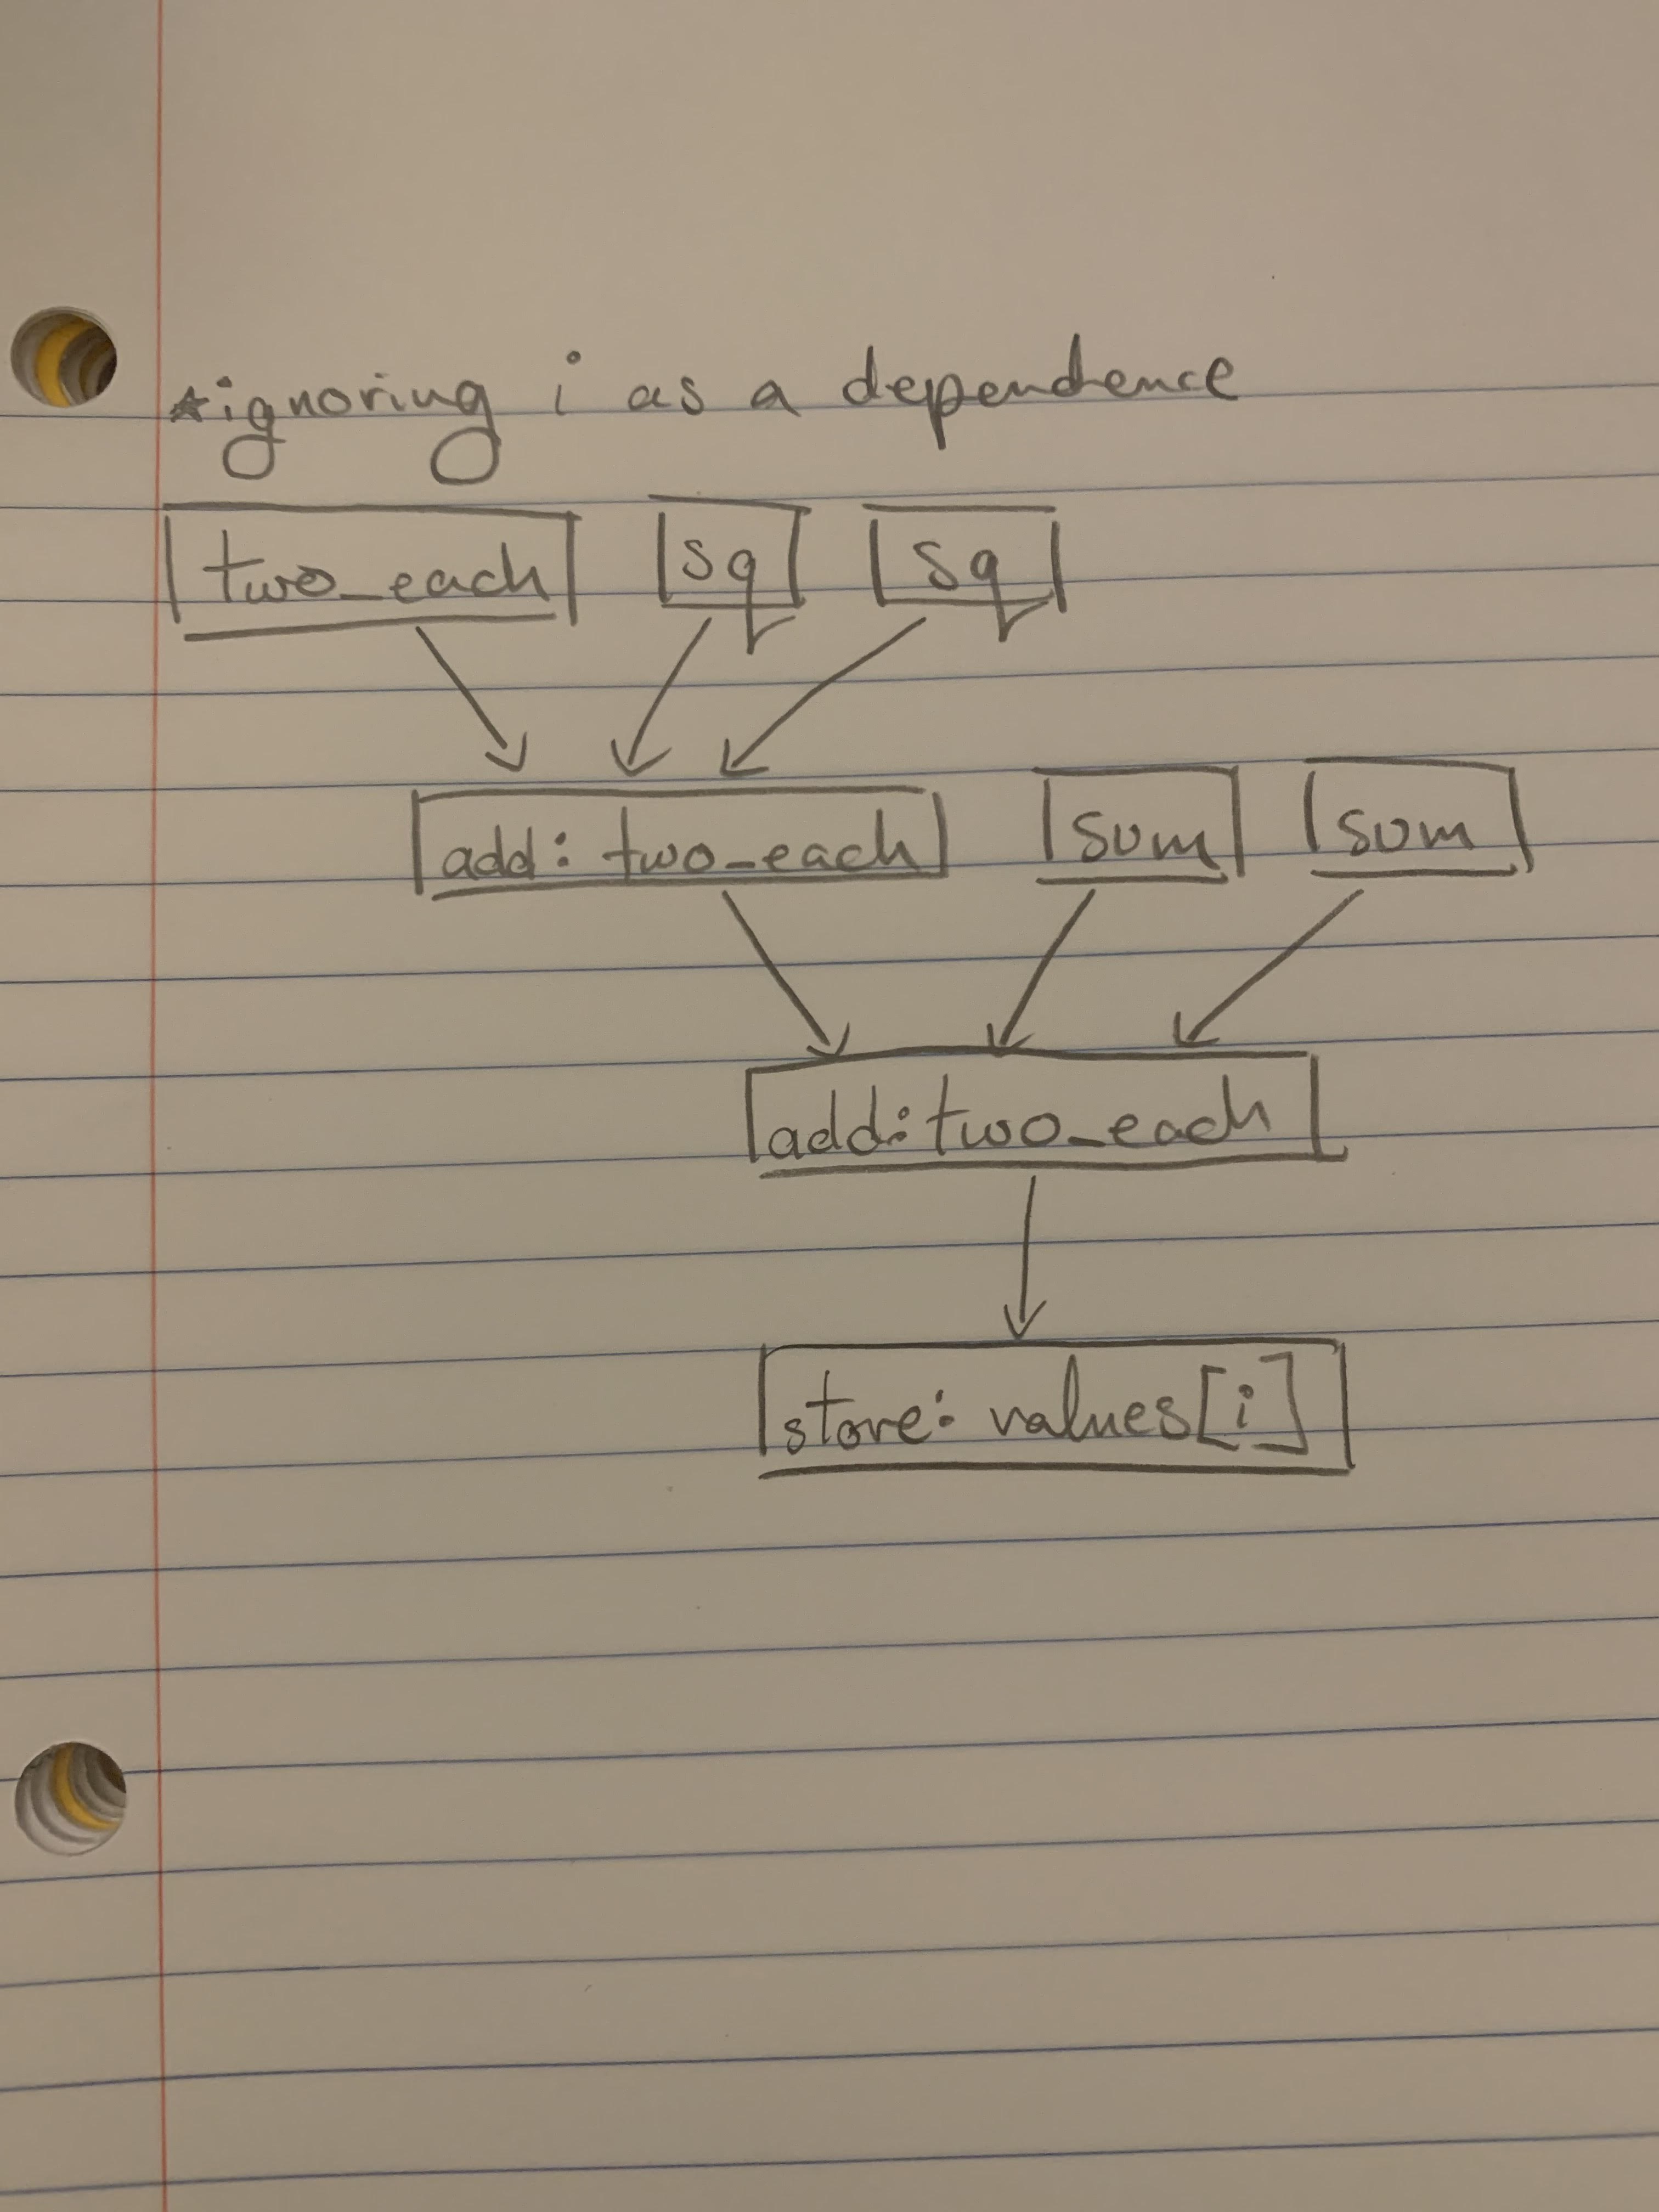
\includegraphics[width=\linewidth]{CS Pic.jpg}
\end{figure}

\begin{lstlisting}
    two_each = two_each + sq + sq; //line 1
    two_each = two_each + sum + sum; //line 2
    values[i] = two_each; //line 3
\end{lstlisting}

With a program that does not use renaming, these statements must occur in order as line 1 then line 2 then line 3. The dependence of these lines for 
each other derives from line 2 using the result of line 1, and line 3 using the result of line 2. The longest patch of dependences, if we were to count 
the "levels" of arrows in the figure provided would be 3. 

\subsection{B}
\textit{Rename one of the program variables to eliminate a dependence, and thereby shorten
the critical path. How much can it be shortened?}
\paragraph{}I chose to rename the $two_each$ of line 1. By renaming the result of line 1 then we effectively treat it as a different value than the second
$two_each$ in line 2. Because the values are different, line 2 no longer depends on line 1 and therefore instruction level parallelism can be exploited. By 
removing the dependence between lines 1 and 2 we shorten the critical path from 3 to 2. 
\subsection{C}
\textit{the i (loop index variables) are technically a dependence from one iteration to the next,
but because the values involve only a simple incremement, a compiler can figure out
how to enable iterations to execute with dependences on each other by substituting a
constant i value for each iteration. For example, the first iteration would get i=0, the
second would get i=1, and so on. However, the dependence in the second loop on the
value sum is not so easily broken. Think about this, explain why the compiler cannot
substitute a value for sum in each iteration?}
\paragraph{} The reason why the compiler cannot just substitute a value for sum in each iteration is because the sum value depends on 
the previous sum value. This dependence on the previous is unlike the increment of i because while it does indeed take a $+ 1$ to get from $i = 2$ 
to $i = 3$, the index variables are really just a list of natural numbers. However, every value of $sum$ at iteration $i$ is used and therefore affects 
the result of $sum$ at iteration $i + 1$. In fact, even in our case we know that $value[i]$ will always be consistently proportional and thus $sum$ will 
also be proportional to its previous and future $sum$. But this cannot always be assumed. An example where a dependence on a previous value would prove really 
important is if $value[i]$ was replaced with $randomValueBetween(1, 1000)$. Thus, each sum at each iteration would have a starkly different result 
dependning on both the previous value and the random value. 

\section{4.11}
\textit{Debugging, code optimization, and sequence. In modern compilers, an extensive
analysis allows the program to be transformed significantly for higher performance. We
have come to depend on these transformations that often produce a program execution
structure quite different from the source program. In short, they can make it difficult to
reconstruct the sequential abstraction view of the program execution. As a result, many
debuggers do not work on optimized programs}

\subsection{A}
\textit{Explain why reconstructing the sequential abstraction can be difficult. Be precise and
give a specific example of a program.}
\paragraph{} Reconstructing the sequential abstraction of a program is difficult because removing dependencies
means the original order of the lines of code is not preserved. For example, if an original program has the order Line 1 then line 2, 
then reconstructing the sequence  means either 1 came before 2 or 2 came before 1. For two lines of code this menas there are 2! options for rearranging. 
However, for more lines of code with more dependencies, the number of permutations for reconstructing the sequential state abstraction drastically rises 
increasing the difficulty.   
\subsection{B}
\textit{Consider instruction-level parallelism, and speculative execution. If a branch is mispredicted, the machine must return the architectural state to the proper values at the
time the branch was executed. How does it do this? Does ensuring that this is possible
place any restrictions on speculation?}
\paragraph{} When a branch fails, it turns to the speculative branch log to return the AS proper values. Since speculative execution keeps a log of which branches it has 
executed (using flags), the registers and memory it has updates (using renaming), all changes can either be committed or erased. Upon an incorrect guess, the execution cancels 
all updates past the failed branch prediction, which loses that work. However, to reset the architectural state back to the last successful execution the log write pointer is 
simply moved back. This works most effectively with a speculative execution log which depending on the amount of registers of the re-order buffer 
restricts how much data it can keep track at any one time. Today's machines have upwards to 256 regissters for speculative execution but nonetheless a finite amount. If it were to run 
out of space, the thread can wait for more space. 
\section{5.5}
\textit{In Section 5.1, we discussed four different memory technologies for storing bits of
information: acoustic waves, magnetic polarization, electric charge, and phase-change to
store bits. Think about other “technologies” that could be used to store bits in a computer.
}
\subsection{A}
\textit{Describe three different ways in which binary information is stored in your everyday
life. For each, describe what a “1” and what a “0” represents, whether it is persistent,
and what causes changes in the value of a bit?}
\subparagraph{Lightbulbs} Lightbulbs are usually one of the first things I think of for binary information. As I understand, a lightbulb has an "on" and "off" binary
which could correspond to "1" and "0" respectively. Oftentimes, the binary information that is stores in lightbulbs is whether of not the bulb has power, but for 
modern devices could also include whether or not it shines color, or whether or not it is scheduled to turn off, for example. Lightbulbs in particular are usualy persistent. 
They are often expected to be left on while in use and off while not. The causes in changes could be the flip of a switch which could divert power to or away from the lightbulb
or even a software application that flips the bulb off even if it has power. 
\subparagraph{Drawing Tablet} My drawing tablet is another good example of bits being stored but is slightly more unique than a lightbulb. To draw using a tablet, the drawing 
tablet registers where on the surface the pen is located and matches that location onto another device or screen. The binary here is whether or not the pen is registered as active
by the tablet: where the pen is located represents a "1" to draw, and where the pen is not located represents a "0" to not draw. However, the drawings of a tablet would be persistent
in the sense that the effect of "1" remains, the drawing does not simply erase. This is unlike a lightbulb where "1" and "0" dictate light or no light but the bits of a drawing tablet just dictate
whether or not the pen is currently updating the drawing. 
\subparagraph{Bluetooth Headphones} Bluetooth connections are also a source of binary information in my everyday life. Devices that can connect and disconnect over bluetooth exemplify 
a binary structure. The "1" bit is represented by a successful connection and the "0" bit is represented by no connection. These connections are also expected to be persistent and bluetooth 
connections are usually manually created or destroyed. This means that usually there's a person enabling the pairing of two or more devices, or a device itself can shut down and disconnect 
another device simultaneously. 
\subsection{B}
\textit{Think about the different ways we have seen to store information for computers such
as punch cards, paper tape, magnetic tape, CD’s, DVD’s, bubble memory and more.
It is important for bits to be small, so that storage can be small. What is the smallest
thing way to store bits that you can think of? Are there fundamental limits?}
\paragraph{} One of the smallest ways to store a bit that i can think of is probably lasers. I can imagine there existing incredibly precise lasers with mechanisms that can exist outside of 
the device but then active storage bits inside a storage space. I could imagine the storage bits are as small as possible to accept the smallest, most precise amount of light. I would 
claim that light hitting the bit would charge it to "1" instantly and no light is a "0". Fundamentally we could get smaller and smaller with the way we store bits, however, as we minitarize the information, we have to begin taking into account the effect of 
minitiarization on the materials we work with. So for my example of lasers, I would think its is difficult to prevent the lasers from activating other bits as the light bleeds. 
\subsection{C}
\textit{Beyond small size, one of the important properties of memory in a computer is fast
read and write operations. For some you proposed above, how long would it take to
read a bit? write a bit?}
\paragraph{}Drawing tablets usually rate their drawing speeds as report rate speed which details the speed at which I could tap on the fill bucket icon in photoshop and have my tool 
become the fill bucket. On average, drawing tablets have about 200 Hz RPS which means drawings and activity on a drawing tablet registers at about 1/200th of a secon, or 5 milliseconds. 
\section{5.9}
\textit{The original 64-bit SRAM memory was approximately 4 cm3
. In this problem we
will compare it to flash memory technologies.}
\subsection{A}
\textit{How does this compare to early NAND Flash memories introduced in 1987?}
\paragraph{}I couldn't really find an exact number for NAND Flash memories of 1987 but the closest area of a memory storage dating back to the 1993s was NOR Flash type of size $280mm^2$
or approximately 28 cm in area. 
\subsection{B}
\textit{Compare its density to modern NAND flash memory chips such as Samsungs 136-
layer 256gbit v-NAND technology? (2019) How much has density increased?}
\paragraph{} For the density of the NAND flash memory chips, there are roughly 670 million holes that create the uniform 3d charge trap flash cells of the device. The NOR flash type of 1993 has a density of 


\section{5.10}
\textit{Despite the rapid increase in memory density, the even faster growth of software’s
appetite for memory has caused memory latency to increase. In fact, the growth of application memory use is the key reason for exploiting dynamic locality. In this problem, we
will explore several reasons for memory demand growth. For each, estimate how much
application memory size may have increased as a result, and explain your estimate.}
\subsection{A}
\textit{Larger computer word sizes (16-bit to current x86 64)}
\paragraph{} Estimation: $64/16 = 4x$ increase in the amount of bits however, $\frac{2^{64}}{2^{16}} = \num{2.8e14}$ increase in unique bit values to store data.
 Considering that word sizes are the most basic unit of a computer, changing the amount of information that can be read/written to and from registers by $\num{2.8e14}$ is 
 incredibly impactful.  
\subsection{B}
\textit{Larger programs – dozens to billions of lines of code}
\paragraph{} Estimation: $\frac{262144}{.0039} = 67,216,410.3$ fold increase. I found these numbers off figure 5.10 of the textbook and compared the amounts of megabytes stored between 
1950 and 2020. I used those data points to calculate my result. 
\subsection{C}
\textit{Higher precision scientific models, for example progress in modeling climate from
256x256 km tiles to 1x1 km tiles}
\paragraph{} $\frac{256^2}{1} = 65 536$ or about the difference between 1 byte and 64 KiB. With higher precision scientific models, climate change across the globe can be tracked and recorded 
more accurately. This would allow scientists to analyze how populations, homes, habitats, and environments down to a 1 by 1 kilometer tile are affected by unnatural climates. 
\subsection{D}
\textit{Larger datasets driven by much higher computer transaction rates - purchaes, web
clicks, web searches, cameras, etc.}
\paragraph{} Today an AMD Ryzen Threaripper 3990x (2020) can run up to 2,356,230 MIPS (millions of instructions per second) which drastcially demands a lot from memory, as the memory bandwidth reads up to
55GB/second.
\subsection{E}
\textit{Larger datasets due to aggregating these very large datasets by internet powerhouses
such as Google and Facebook}
\paragraph{} Google Chrome currently is using up 6,096 MB or 82\% of my current RAM with 2.8 GB cached. The memory demand from the web browser is a lot but it provides so much through 
internet searches, applications, downloading, security, accounts and history, etc.   
\section{Extra Credit}
\paragraph{} I had some trouble with PSET problems 5.9 and 5.10 because I still didn't really grasp the concepts of calculating memory usage. Finding the right values of memory for devices 
like the NAND flash memory of 1987 is fairly difficult. It would be easier if there was a table of values we could pull from, like Table 5.1 in the textbook, where we can then focus
on the computations necessary to see the difference. Having to search for values I oftentimes am not confident are right takes away from the impact of computing the architectural differences. 


\end{document}
